% -*- root: ../../../main.tex -*-
\subsection{Basics}
Un cluster RAFT può contenere vari server, solitamente cinque è il numero tipico, questo permette al sistema di tollerare due fallimenti.
  \subsubsection{Stati di un server}
  Abbiamo tre stati in cui si può trovare generalmente un server:
  \begin{itemize}
    \item{\textbf{Leader:}}
    In operazioni normali esiste esattamente \textbf{un solo leader} mentre i rimanenti sono followers. Quando il leader viene eletto allora esso ha \textbf{pieno potere} e tutti i rimanenti follower devono seguire i suoi ordini.\\
    Il leader solitamente ha due compiti fondamentali:
    \begin{itemize}
      \item{\emph{Gestione delle richieste da parte dei client}} 
      \item{\emph{Replicazione del log}}
    \end{itemize}
    \item{\textbf{Follower:}}
    I follower sono server totalmente \textbf{passivi}, essi intraprendono due azioni fondamentali: 
    \begin{itemize}
      \item{\emph{Risposta alle richieste di leader e candidate}}
      \item{\emph{Redirection al leader delle richieste da parte dei client}}
      \item{\emph{Se non hanno più notizie dal leader da un po' allora diventano ``ansiosi'' e diventano candidate}}
    \end{itemize}
    \item{\textbf{Candidate:}}
    Lo stato di candidate è usato per \textbf{eleggere un nuovo leader}.
  \end{itemize}
  L'immagine \ref{fig:figure2} qua sotto mostra come avvengono le transizioni fra i vari stati.

  \begin{figure}[H]
    \centering
    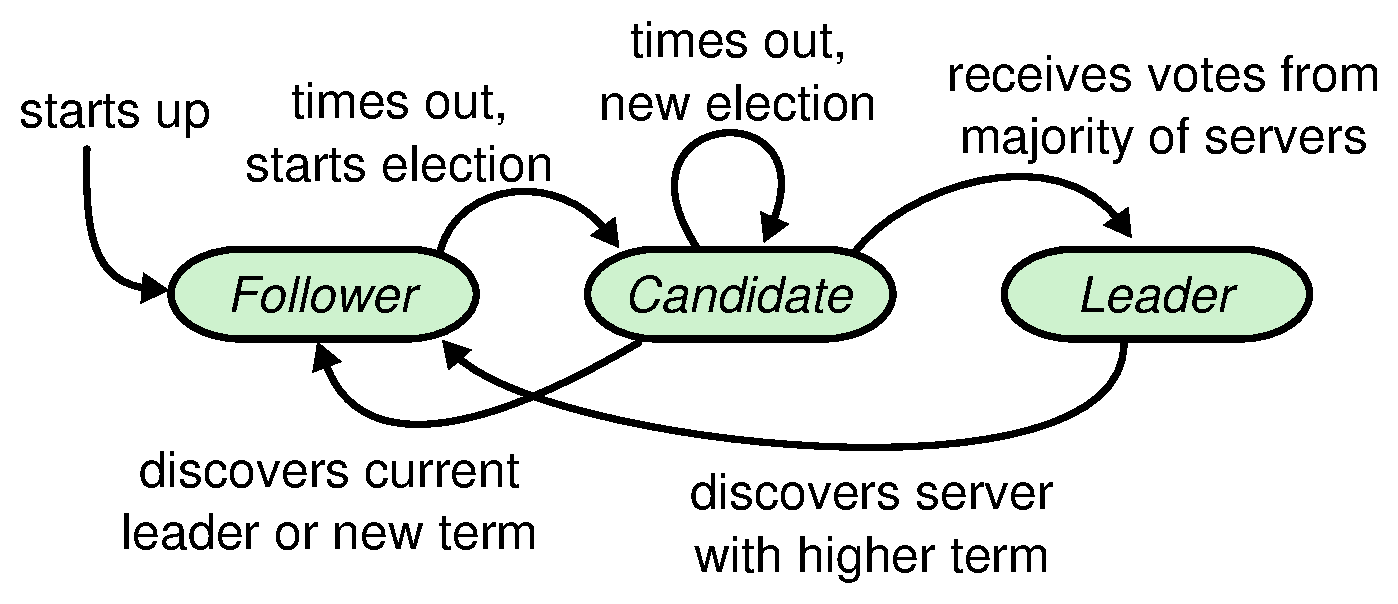
\includegraphics[width=0.90\columnwidth]{raft/followercandidateleader.pdf}
    \caption{Diagramma a stati che descrive il passaggio di stato dei singoli server}
    \label{fig:figure2}
  \end{figure}

  \subsubsection{Terms}
  IL tempo in RAFT è diviso in periodi di \textbf{lunghezza arbitraria} chiamati \textbf{terms}. I term godono di queste proprietà:
  \begin{itemize}
    \item{\textbf{Identificativo:}}
    A ciascun term è associato un numero in modo \textbf{incrementale} e \textbf{assoluto} nel tempo.
    \item{\textbf{Leader-centric:}}
    Ogni term parte con l'elezione di \textbf{uno e un solo leader}: se l'elezione ha successo allora il candidate eletto avrà potere per tutta la durata del term. Può capitare che più candidate provino a diventare leader nello stesso instante: in questo caso il risultato della votazione premierà un solo candidate. Raft garantisce che non ci sia più di un leader per term.
    \item{\textbf{Leader-less}}
    In alcuni casi può capitare che nessun leader emerga, questo avviene perché nella votazione non è stata ottenuta una maggioranza assoluta. In questo caso si dice che è avvenuto un \textbf{vote-split} e al fine di garantire safety \textit{nessun leader può essere eletto}.\\
    In questo caso l'algoritmo considererà l'elezione come \textbf{failed} e verrà aperta immediatamente una \textbf{nuova elezione}.
    \item{\textbf{Term come logical clock}}
    I term in RAFT hanno uno scopo molto più generale oltre al contesto dell'elezione: essi agiscono come \textbf{logical clock} \cite{Lamport:1978} garantendo un concetto logico di tempo. e garantendo ai server di accorgesi quando sono in possesso di \textbf{informazioni obsolete}.
  \end{itemize}
    \paragraph{Identificazione di informazioni obsolete}
    Non esiste in RAFT un concetto di stato/term globale ma ogni \textbf{server vede}, in un \textbf{dato istante}, una \textbf{parte del sistema} e non è detto che sia lo stesso per tutti.\\
    L'identificazione di informazioni obsolete avviene in modo molto semplice:
    \begin{enumerate}
      \item Ogni server contiene al suo interno le informazioni sul \textbf{term attuale} che ovviamente può incrementare nel tempo in modo monotonico.
      \item Nel momento in cui avviene una comunicazione ogni server \textbf{include} nel proprio \textbf{messaggio} anche le informazioni sul \textbf{proprio term}.
      \item Nel caso in cui un server si accorge di avere un term troppo obsoleto \textbf{aggiorna} immediatamente il proprio \textbf{term} con quello più \textbf{recente}.
      \begin{itemize}
        \item Se il server si trova nello stato di leader allora esso \textbf{regredisce} immediatamente \textbf{a follower}
      \end{itemize}
      \item Se un server riceve messaggi con \textbf{term obsoleti} questi vengono immediatamente \textbf{rifiutati}.
    \end{enumerate}

  



